\documentclass[a4paper,10pt]{scrreprt}
	\usepackage{sty/package}
	\usepackage{sty/document}
	\usepackage{sty/math}
	\usepackage{chngcntr}
	\usepackage{mathtools}
	\usepackage{algorithm2e}
	\usepackage{enumitem}
	\usepackage{graphicx}
	\usetikzlibrary{positioning}
	\usetikzlibrary{arrows}

	\lstset{
	basicstyle=\ttfamily,
	mathescape
	}
	\setlength\parindent{0pt}
	
	\pagestyle{fancy}
	\fancyhead[R]{Netzwerkalgorithmen}
	
	\counterwithout{section}{chapter}
	\counterwithin{figure}{section}
	\setcounter{chapter}{1}
	
	\renewcommand{\labelitemi}{$-$}
	
	\renewcommand*{\algorithmcfname}{Algorithmus}
	\RestyleAlgo{boxed}
	\LinesNumbered
	\SetKwInOut{Input}{Eingabe}
	\SetKwInOut{Output}{Ausgabe}

\begin{document}
	\section{Graphen}
	\begin{definition}[Ungerichteter Graph]
		Ein \textbf{ungerichteter Graph} $G$ ist ein Tripel $(V, E, \Psi)$, für das
		\begin{enumerate}
			\item $V$ und $E$ endliche Mengen sind und
			\begin{itemize}
				\item $V$ ist die Knotenmenge
				\item $E$ ist die Kantenmenge
			\end{itemize}
			\item $\Psi$ eine Funktion mit
			\begin{equation*}
				\Psi : E \to \set{X \subseteq V \vert 1 \le \card{X} \le 2}
			\end{equation*}
			ist.\\
		\end{enumerate}
		\begin{itemize}
				\item Zwei Kanten $e, e'$ sind \textbf{parallel}, wenn $\Psi(e) = \Psi(e')$.
				\item Eine Kante $e$ ist eine \textbf{Schleife}, falls $\card{\Psi(e)} = 1$.
				\item Ein Graph ohne parallele Kanten und Schleifen heißt \textbf{einfach}. Man schreibt dann $G = (V, E)$ mit $E(G)$ der Kantenmenge von G.
				\begin{itemize}[label=$\hookrightarrow$]
					\item  In einem einfachen Graphen kann man $\set{v_i, v_j}$ für eine Kante $e_{i,j}$ zwischen $v_i$ und $v_j$ schreiben.
				\end{itemize}
				\item $\card{E}$ ist die Zahl der Kanten und $\card{V}$ die Zahl der Knoten von $G$.
				\begin{itemize}[label=$\hookrightarrow$]
					\item Oft verwendet man $n$ für $\card{V}$ und $m$ für $\card{E}$.
				\end{itemize}
			\end{itemize}
	\end{definition}
	\begin{definition}[Nachbarschaft in Graphen]
		Eine Kante $e = \set{v, w}$ in einem Graphen verbindet zwei Knoten $v$ und $w$. Der Knoten $v$ ist dann Nachbar von $w$, d.h. $v$ und $w$ sind \textbf{adjazent} (\dq benachbart\dq). Außerdem ist sowohl $v$ als auch $w$ \textbf{inzident} (\dq zusammentreffend mit\dq) zu $e$.
	\end{definition}
	\begin{definition}[Knotengrad]
		Der \textbf{Grad} eines Knotens $v$ ist die Anzahl der inzidenten Kanten und wird bezeichnet mit $deg(v)$ (auch $\delta(v)$).\\[5pt]
		Ein Knoten $v$ heißt \textbf{isoliert}, wenn $deg(v) = 0$.
	\end{definition}
	\begin{satz}
		Sei $G = (V, E)$ ein Graph. Dann gilt
		\begin{equation*}
			\sum_{v \in V} deg(v) = 2\card{E}.
		\end{equation*}
		D.h. die Summe über alle Knotengrade ist gleich 2-mal die Anzahl der Kanten.
	\end{satz}
	\begin{lemma}[Handshake-Lemma]
		In jedem Graphen ist die Anzahl der Knoten mit ungeradem Grad gerade.
	\end{lemma}
	\begin{definition}[Teilgraph]
		Ein Teilgraph $H = (V(H), E(H))$ eines Graphen $G =\\ (V(G), E(G))$ ist ein Graph mit
		\begin{eqnarray*}
			V(H) &\subseteq& V(G),\\
			E(H) &\subseteq& E(G).
		\end{eqnarray*}
		$H$ ist \textbf{aufspannend}, wenn $V(H) = V(G)$ gilt.
	\end{definition}
	\begin{definition}[Isomorph]
		Seien $G = (V(G), E(G))$ und $H = (V(H), E(H))$ zwei Graphen. Wenn es eine bijektive Abbildung $f : V(G) \to V(H)$ gibt, sodass $\set{v, w} \in E(G)$ gilt, genau dann, wenn $\set{f(v), f(w)} \in E(H)$ gilt, dann nennen wir die Graphen \textbf{äquivalent} (oder \textbf{isomorph}).
	\end{definition}
	
	\subsection{Datenstrukturen für Graphen}
	\begin{definition}[Adjazenzmatrix]
		Eine \textbf{Adjazenzmatrix} $A = (a_{vw})$ eines Graphen $G = (V, E)$ beschreibt, welche Knoten $v_i$ zu welchen Knoten $v_j$ adjazent sind ($v_i, v_j \in V$). Die Matrix hat die Dimension $n\times n$, wobei $n = \card{V}$.\\
		Es gilt $A\in \set{0, 1}^{n\times n}$ mit
		\begin{equation*}
			a_{vw} := \begin{cases*}
				1 \text{ für } \set{v,w} \in E\\
				0 \text{ sonst}
			\end{cases*}
		\end{equation*}
		Eine Adjazenzmatrix ist quadratisch und symmetrisch. Für einfache Graphen enthält die Diagonale ausschließlich Nullen.\\
	\end{definition}
	\begin{definition}[Inzidenzmatrix]
		Eine \textbf{Inzidenzmatrix} $A = (a_{ve})$ eines Graphen $G = (V, E)$ beschreibt, welche Knoten $v_i \in V$ zu welchen Kanten $e_j \in E$ inzident sind. Die Matrix hat die Dimension $n\times m$, wobei $n = \card{V}$ und $m = \card{E}$.\\
		Es gilt $A\in \set{0, 1}^{n\times m}$ mit
		\begin{equation*}
			a_{ve} := \begin{cases*}
			1 \text{ für } v \in e\\
			0 \text{ sonst}
			\end{cases*}
		\end{equation*}
		Für große Graphen enthält die Matrix tendenziell viele Nullen.
	\end{definition}
	\begin{definition}[Kantenliste]
		Eine \textbf{Kantenliste} eines Graphen $G = (V, E)$ ist eine Liste aus zweielementigen Knotenmengen $\set{v_i, v_j} \in E$, die eine Kante von $v_i$ zu $v_j$ beschreiben $(v_i, v_j \in V)$.\\ Die Kantenliste benötigt $\Theta(m~log(n))$ Speicherplatz und ist damit sparsamer als die Inzidenzmatrix (für $n \ge 8$).
	\end{definition}
	\begin{definition}[Adjazenzliste]
		Eine \textbf{Adjazenzliste} eines Graphen $G = (V, E)$ gibt zu jedem Knoten $v_i$ die benachbarten Knoten $v_j$ an $(v_i, v_j \in V)$.\\
		Das ist etwas praktischer als die Kantenliste, wenn man für Graphenalgorithmen direkten Zugriff auf die Nachbarn eines Knotens benötigt. Man muss nicht die Nachbarn erst mühsam aus einer Liste heraussuchen.\\
		Die Adjazenzliste benötigt $\Theta(n~log(n)+m~log(n))$ Speicherplatz. Im Allgemeinen sind Graphen mit vielen isolierten Knoten (ohne Kanten) uninteressant, d.h z.B. $m\ge \frac{n}{2}$ oder $m\ge n$ o.ä. Also wieder $\Theta(m~log(n))$.
	\end{definition}
	
	\subsection{Wege und Pfade}
	\begin{definition}[Kantenfolge]
		Eine \textbf{Kantenfolge} $W$ in einem Graphen $G = (V, E)$ ist eine Folge $v_1, e_1, v_2, e_2, v_3, ..., e_k, v_{k+1}$ mit $k \ge 0,~e_i = \set{v_i, v_{i+1}} \in E$
	\end{definition}
	\begin{definition}[Weg]
		Wiederholt sich keine Kante in einer Kantenfolge, dann spricht man von einem \textbf{Weg}. Ein \textbf{geschlossener Weg} (auch Tour) kehrt am Ende zum Startknoten zurück. Ein \textbf{Eulerweg} benutzt alle Kanten eines Graphen. Eine \textbf{Eulertour} kehrt außerdem zum Startknoten zurück.
	\end{definition}
	\begin{definition}[Pfad]
		Wiederholt sich kein Knoten in einer Kantenfolge, dann sprichtman von einem \textbf{Pfad}. Ein \textbf{Kreis} ist ein geschlossener Pfad, d.h. der Pfad kehrt zum Startknoten zurück. Ein \textbf{Hamiltonpfad} besucht alle Knoten eines Graphen. Ein \textbf{Hamiltonkreis} (auch Hamiltontour) kehrt außerdem zum Startknoten zurück.
	\end{definition}
	\begin{satz}
		Sei $G$ ein Graph mit Adjazenzmatrix $A$. Der Koeffizient $a_{vw}^{(m)}$ von $A^m$ gibt die Anzahl der Kantenfolgen der Länge $m$ von Knoten $v$ zu Knoten $w$ an. Insbesondere gilt $a_{vv}^{(2)} = deg(v)$.
	\end{satz}
	\begin{definition}[Zusammenhängend]
		Ein Graph $G$ heißt \textbf{zusammenhängend}, wenn es zwischen je zwei Knoten aus $G$ einen Weg gibt.\\[5pt]
		Ein maximaler zusammenhängender Teilgraph von $G$ heißt eine \textbf{(Zusammenhangs-) Komponente} von $G$.
	\end{definition}
	\begin{satz}[notwendiges Kriterium]
		Ein zusammenhängender Graph $G$ mit $n$ Knoten muss zumindest $n - 1$ Kanten haben.
	\end{satz}
	\begin{satz}[hinreichendes Kriterium]
		Ein Graph $G$ mit mehr als $\frac{(n-1)(n-2)}{2}$ Kanten ist zusammenhängend.
	\end{satz}
	\begin{problem}[Zusammenhang]~\\[5pt]
		\hspace*{10pt}\textbf{Gegeben: } Ein Graph $G = (V, E)$.\\[5pt]
		\hspace*{10pt}\textbf{Gesucht: } Ist $G$ zusammenhängend?
	\end{problem}
	\begin{algorithm}[H]
		\Input{Graph $G$}
		\Output{Ist $G$ zusammenhängend}\vspace*{5pt}
		Markiere einen beliebigen Startknoten.\\
		Für jeden im voherigen Schritt markierten Knoten: Markiere alle noch nicht markierten adjazente Knoten. Wurde kein neuer Knoten markiert, dann 3. Sonst wiederhole 2.\\
		Sind noch unmarkierte Knoten übrig \Return \dq $G$ ist nicht zusammenhängend\dq. Sonst \dq$G$ ist zusammenhängend\dq.
		\caption{Algorithmus zum Entscheiden ob ein Graph $G$ zusammenhängend ist. Laufzeit: $O(\card{E})$}
	\end{algorithm}
	\begin{satz}
		Ein Graph $G$ mit Adjazenzmatrix $A$ ist zusammenhängend, genau dann, wenn
		\begin{equation*}
			Z = I_n + A + A^2 + ... + A^{n-1} \text{ mit } z_{vw} \neq 0~ \forall v, w \in \set{1, ..., n}
		\end{equation*}
		existiert.
	\end{satz}

	\subsection{Eulerwege und Hamiltonpfade}
	\begin{problem}[Eulerweg]~\\[5pt]
		\hspace*{10pt}\textbf{Gegeben: } Ein Graph $G = (V, E)$.\\[5pt]
		\hspace*{10pt}\textbf{Gesucht: } Ein Eulerweg $W$ in $G$ -  oder ein Argument, dass kein Eulerweg existiert.
	\end{problem}
	\begin{satz}
		Ein Graph $G = (V, E)$ besitzt genau dann einen Eulerweg, wenn es höchstens zwei Knoten mit ungeradem Grad gibt.
	\end{satz}
	\begin{algorithm}
		\Input{Graph $G$}
		\Output{Ein Weg in $G$}\vspace*{5pt}
		Starte in einem Knoten $v_0$ \newline(wenn einer mit ungeradem Grad existiert, dort, sonst beliebig)\\
		$i \leftarrow 0$\\
		\While{es gibt eine zu $v_i$ inzidente Kante}
		{wähle eine zu $v_i$ inzidente, unbenutze Kante $\set{v_i, v_j}$\\
		laufe zum Nachbarknoten $v_j$\\
		lösche $\set{v_i, v_j}$ aus der Menge der unbenutzen Kanten\\
		$v_{i+1} \leftarrow v_j$\\
		$i \leftarrow i+1$
		}
		\caption{Algorithmus zum Finden eines Weges in einem Graphen}
	\end{algorithm}
	\begin{satz}
		Wenn der Algorithmus 2 stoppt, bleibt ein eulerscher Graph zurück, d.h. ein Graph mit lauter Knoten geraden Grades.
	\end{satz}
	\begin{korollar}~
		\begin{enumerate}
			\item Zwei geschlossene Wege mit einem gemeinsamen Knoten kann man in einen geschlossenen Weg verwandeln.
			\item Man kann aus allen Wegen einen Weg machen, wenn der Graph zusammenhängend ist, indem man immer wieder 1. anwendet.
		\end{enumerate}
	\end{korollar}
	\begin{algorithm}
		\Input{Zusammenhängender Graph $G$ mit höchstens 2 ungeraden Knoten}
		\Output{Ein Eulerweg, bzw. eine Eulertour in $G$}\vspace*{5pt}
		Starte in einem Knoten $v$ \newline(wenn einer mit ungeradem Grad existiert, dort, sonst beliebig)\\
		verwende Algorithmus 2, um einen Weg $W$ von $v$ aus zu bestimmen\\
		\While{es existieren unbenutzte Kanten}
		{wähle einen Knoten $w$ aus $W$ mit positivem Grad im Restgraphen\\
		verwende Algorithmus 2, um einen Weg $W'$ von $w$ aus zu bestimmen\\
		verschmelze $W$ und $W'$\\
		}
		\caption{Algorithmus zum Finden eines Eulerweges oder einer Eulertour}
		\label{fig:Algorithmus}
	\end{algorithm}
	\begin{algorithm}[H]
		\Input{Zusammenhängender Graph $G$ mit höchstens 2 ungeraden Knoten}
		\Output{Ein Eulerweg, bzw. eine Eulertour in $G$}\vspace*{5pt}
		Starte in einem Knoten $v_0$ \newline(wenn einer mit ungeradem Grad existiert, dort, sonst beliebig)\\
		$i \leftarrow 0$\\
		\While{es gibt eine zu $v_i$ inzidente, unbenutzte Kante}
		{wähle eine dieser Kanten $\set{v_i, v_j}$, die den Restgraph zshgd. lässt\\
		laufe zum Nachbarknoten $v_j$\\
		markiere $\set{v_i, v_j}$ als benutzt\\
		$v_{i+1} \leftarrow v_j$\\
		$i \leftarrow i+1$
		}
		\caption{Algorithmus von Fleury zum Finden eines Eulerweges oder einer Eulertour}
	\end{algorithm}
	\begin{satz}[hinreichendes Kriterium]
		Wenn ein Graph mit $n$ Knoten mindestens $\frac{1}{2}(n-1)(n-2)+2$ Kanten hat, dann besitzt er einen Hamiltonkreis.
	\end{satz}

	\section{Minimale aufspannende Bäume}
	\begin{problem}[minimaler aufspannender Baum / kürzestes zsgd.es Netzwerk]~\\[5pt]
		\hspace*{10pt}\textbf{Gegeben: } Ein Graph $G = (V, E)$, Gewichtfunktion
		\begin{eqnarray*}
			c : E &\to& \reell_+\\
			e &\mapsto& c_e
		\end{eqnarray*}
		\hspace*{10pt}\textbf{Gesucht: } Eine Kantenmenge $F\subseteq E$ mit möglichst geringen Gesamtgewicht $\sum_{e \in F} c_e$, \hspace*{60pt}so dass in $T = (V, F)$ alle Knoten verbunden sind ODER entscheide, dass \hspace*{56pt} $G$ nicht zshgd. ist.
	\end{problem}\vspace*{10pt}
	\begin{enumerate}
		\item Welche Eigenschaften haben Lösungen?\\
		$\hookrightarrow$Struktur
		\item Wie findet man optimale Lösungen?
		\item Können wir algorithmische Grundideen verwenden, die auch in anderen Situationen funktionieren?
		\item Effizienz
	\end{enumerate}
	\begin{beobachtung*}
		Ein optimale Lösung für Problem 2.1 kann kein Kreis enthalten. (Beweisskizze: Entfernt man aus einem Kreis eine Kante bleibt der Rest immer noch verbunden).
	\end{beobachtung*}
	\begin{satz}
		Eine optimale Lösung für Problem 2.1 ist zusammenhängend und kreisfrei, also ein Baum.
	\end{satz}
	\begin{proof}
			Klar.
	\end{proof}
	Wir betrachten Eigenschaften von Bäumen. Wie viele Kanten hat ein Baum mit $n$ Knoten? Mit jeder eingefügten Kante nimmt die Zahl der Zhk. um 1 ab (mit jeder gelöschten um 1 zu).
	\begin{beobachtung*}
		Ein Baum mit $n$ Knoten hat $n-1$ Kanten. ABER: Nicht jeder Graph mit $n-1$ Kanten und $n$ Knoten ist ein Baum.
	\end{beobachtung*}
	\begin{definition}
		Für einen Graphen $G$ und $X,Y\subseteq V(G)$ ist
		\begin{eqnarray*}
			E(X,Y) &=& \set{\set{x,y}\in E(G)\vert x \in X\setminus Y,~y \in Y\setminus X}\\
			E^+(X,Y) &=& \set{(x,y)\in E(G)\vert x \in X\setminus Y,~y \in Y\setminus X}
		\end{eqnarray*}
		Für einen ungerichteten Graphen $G$ und $X \subseteq V(G)$
		\begin{equation*}
			\delta(X) = E(X, V(G)\setminus X)
		\end{equation*}
		Für einen gerichteten Graphen $G$ und $X\subseteq V(G)$
		\begin{eqnarray*}
			\delta^+(X) &=& E^+(X, V(G)\setminus X)\\
			\delta^-(X) &=& \delta^+(V(G)\setminus X)\\
			\delta(X) &=& \delta^+(X) \cup \delta^-(X)
		\end{eqnarray*}
	\end{definition}
	\begin{lemma}~
		\begin{enumerate}[a)]
			\item Ein ungerichteter Graph $G$ ist zusammenhängend $\Leftrightarrow \delta(X) \neq \emptyset~ \forall ~\emptyset \neq X \subset V(G)$.
			\item Sei $G$ ein gerichteter Graph und $r \in V(G)$. Dann gibt es einen Pfad von $r$ nach $v$ für jeden $v \in V(G) \Leftrightarrow \delta^+(X) \neq \emptyset~\forall~X\subset V(G)$ mit $r\in X$.
		\end{enumerate}
	\end{lemma}
	\begin{proof}
		
	\end{proof}
	
	\section{Kürzeste Wege}
\begin{problem}~\\[5pt]
	\hspace*{10pt}\textbf{Gegeben: }Gerichteter Graph $G$, Gewichte $c:A(G)\to \reell$, zwei ausgezeichnete \hspace*{60pt} Knoten $s,~t$.\\[5pt]
	\hspace*{10pt}\textbf{Gesucht: }$s$-$t$-Pfad minimalen Gesamtgewichts.
\end{problem}
Verschiedene Schwierigkeitsstufen
\begin{itemize}
	\item alle Kanten Einheitslänge $c(a)=1~ \forall a\in A(G)$.\\
	$\hookrightarrow$ (BFS) Suche nach Pfad mit minimaler Anzahl an Kanten.
	\item nicht negative Kantenlängen.\\
	$\hookrightarrow$ Dijkstra.
	\item ohne Kreise negativen Gesamtgewichts.
	\item allgemeine Kantengewichte.
\end{itemize}
\begin{definition*}[Konservativ]
	Sei $G$ ein Graph mit Gewichten $c:E(G)\to \reell$. Diese Kantengewichtsfunktion heißt konservativ wenn sie keine Kreise negativen Gesamtgewichts enthält.
\end{definition*}
\subsection{Kürzeste Wege von einer Quelle}
	\section{Netzwerkflüsse}
\textit{Flüsse in Graphen. Beispiele:
\begin{itemize}
	\item Wasser in Leitungssystemen
	\item Verkehr in Straßensystemen
	\item Passagiere in Transportsystemen
\end{itemize}
Eigenschaften:
\begin{itemize}
	\item pro Kante 2 Kenngrößen
	\begin{itemize}
		\item mögliche Flusskapazität
		\item tatsächlicher Fluss
	\end{itemize}
	\item \dq Flusserhaltung\dq : Bilanzierung der Flüsse an jedem Knoten (\dq fliest nicht mehr raus, als rein\dq)
\end{itemize}}
\begin{definition}
	Gegeben: Digraph $G$ mit Kapazität $u: A(G) \to \reell_+$.
	\begin{enumerate}
		\item Ein \textbf{Fluss} ist eine Funktion $f: A(G) \to \reell_+$ mit $f(e) \le u(e)~\forall e\in A(G)$.
		\item An einem Knoten $v$ gilt \textbf{Flusserhaltung}, wenn \[\sum_{e\in \delta^-(v)} f(e) = \sum_{e\in \delta^+(v)} f(e).\]
		\item Eine \textbf{Zirkulation} ist ein Fluss für den an jedem Knoten Flusserhaltung gilt.
		\item Für ein Netzwerk $(G, u, s, t)$ ist ein Fluss ein $s$-$t$-Fluss, wenn Flusserhaltung an allen Knoten außer $s$ und $t$ gilt \[Wert(f) :=\sum_{e\in \delta^+(s)} f(e) - \sum_{e\in \delta^-(s)} f(e).\]
	\end{enumerate}
\end{definition}
\begin{problem}[Maximaler Fluss]~\\[5pt]
\hspace*{10pt}\textbf{Gegeben: }Netzwerk $(G, u, s, t)$.\\[5pt]
\hspace*{10pt}\textbf{Gesucht: }Ein $s$-$t$-Fluss mit maximalem Wert.
\end{problem}
\textit{Formulierung als LP (Lineares Programm):
\begin{eqnarray*}
	max~ F \text{ sodass} &&\sum_{e\in \delta^+(s)} f_e - \sum_{e\in \delta^-(s)} f_e = F,\\
	&&\sum_{e\in \delta^-(v)} f_e - \sum_{e\in \delta^+(v)} f_e = 0~\forall v\in V(G)\setminus \set{s,t},\\
	&&0\le f_e \le u_e~\forall e\in A(G).
\end{eqnarray*}
Also: Können wir effizient lösen (LP $\in$ P).\vspace*{5pt}\\
Ziel hier: \dq kombinatorische\dq Algorithmen.}
\begin{beobachtung}
	Das Max Flow Problem hat immer eine optimale Lösung.
\end{beobachtung}
\begin{proof}~
	\begin{enumerate}
		\item LP ist beschränkt.
		\item Fluss mit $f\equiv 0$ ist immer zulässig.
	\end{enumerate}
\end{proof}
\begin{definition}
	In einem Digraph $G$ heißt eine Kantenmenge $\delta^+(X)$ mit $s\in X$ und $t\notin X$ ein \textbf{$s$-$t$-Schnitt}.
	Wert des Schnittes := Summe der Kantenkapazitäten der ausgehenden Kanten.
\end{definition}
\begin{lemma}[Schranken durch Schnitte]
	Für bel. $A\subseteq V(G)$ mit $s\in A$, $t\notin A$ und jedem $s$-$t$-Fluss $f$ gilt
	\begin{enumerate}[label=\alph*)]
		\item $Wert(f) = \sum_{e\in \delta^-(A)} f(e) - \sum_{e\in \delta^+(A)} f(e)$
		\item $Wert(f) \le \sum_{e\in \delta^+(A)} f(e)$
	\end{enumerate}
\end{lemma}
\begin{proof}
	zu a): Flusserhaltung gilt für $v\in A\setminus \set{s}$, daraus folgt
	\begin{eqnarray*}
		Wert(f) &=& \sum_{e\in \delta^+(s)} f(e) - \sum_{e\in \delta^-(s)} f(e)\\
		&=& \sum_{v\in A}(\sum_{e\in \delta^+(v)} f(e) - \sum_{e\in \delta^-(v)} f(e))\\
		&=& \sum_{e\in \delta^+(A)} f(e) - \sum_{e\in \delta^-(A)} f(e).
	\end{eqnarray*}
	zu b): Folgt mit a), wenn wir $0 \le f(e) \le u(e)~\forall e\in A(G)$ nutzen.
\end{proof}
\textit{Was sagt Lemma 4.5:\\[5pt]
Der Wert eines Max Flow kann die Kapazität eines minimalen $s$-$t$-Schnitts nicht überschreiben - tatsächlich gilt Gleichheit, zeigen wir später.\\[5pt]
Grundkonzept für Algorithmen: Flüsse erhöhen oder verringern. Interpretation: Fluss verringern $\widehat{=}$ Fluss umleiten.}
\begin{definition}~
	\begin{enumerate}
		\item Für ein Digraph $G$ ist $\overset{\leftrightarrow}{G} := (V(G), A(G) \dot\cup \set{\overset{\leftarrow}{e} \vert e \in A(G)})$ mit $\overset{\leftarrow}{e} = (w,v)$ für $e=(v,w)$ \dq Rückwärtskante\dq~ von $e$ der doppelt gewichtete Graph für $G$.
		\item Für einen Fluss $f$ in einem Digraph $G$ mit Kapazität $z:A(G)\to \reell_+$ definieren wir die \textbf{Residualkapazitäten} $u_f$ \[ u_f(e) = \begin{cases} u(e) - f(e) &\text{für Vorwärtskante,}\\ f(e) &\text{für Rückwärtskante.} \end{cases} \]
		\item Der \textbf{Residualgraph} $G_t$ ist der Graph $(V(G), \set{e\in A(\overset{\leftrightarrow}{G})~\vert~ u_f(e) > 0})$.
		\item Interpretation des Residualgraphen:
		\begin{itemize}
			\item $u_f$ auf Vorwärtskante: um wie viel wir $f$ noch erhöhen können.
			\item $u_f$ auf Rückwärtskante: um wie viel wir $f$ noch verringern können.
		\end{itemize}
	\item Gegeben ein Fluss $f$ und ein Pfad (oder Kreis) $P$ in $G_f$. Um $f$ entlang $P$ um $\gamma$ zu augmentieren muss man
	\begin{itemize}
		\item den Fluss für jede Vorwärtskante um $\gamma$ erhöhen ($e\in A(P)$: wenn $e \in A(G)$, erhöhe $f(e)$ um $\gamma$)
		\item den Fluss für jede Rückwärtskante um $\gamma$ reduzieren ($e \in A(P)$: wenn $e = \overset{\leftarrow}{e_0}$ für $e_0 \in A(G)$, reduziere $f(e_0)$ um $\gamma$)
	\end{itemize}
	\item Ein \textbf{$f$-augmentierender} Pfad in einem Netzwerk $(G, u, s, t)$ mit einem Fluss $f$ ist ein $s$-$t$-Pfad im Residualgraph $G_f$.
	\end{enumerate}
\end{definition}
\begin{algorithm}
	\Input{Netzwerk $(G, u, s, t)$}
	\Output{Ein $s$-$t$-Fluss $f$ mit maximalem Wert}\vspace*{5pt}
	Setze $f(e)=0~\forall e\in A(G)$\\
	Finde einen $f$-augmentierenden Pfad $P$\\
	\hspace*{15pt}Falls keiner existiert: \textbf{stop} \\
	Berechne $\gamma := \underset{e\in P}{min}~ u_f(e)$\\
	\hspace*{15pt}Augmentiere $f$ entlang $P$ um $\gamma$ und \textbf{goto} 2
	\caption{Ford-Fulkerson Algorithmus}
	\label{fig:Algorithmus}
\end{algorithm}
\begin{satz}
	Ein $s$-$t$-Fluss ist optimal $\Leftrightarrow$ Es gibt keinen $f$-augmentierenden Pfad.
\end{satz}
\textit{Also: stoppt der Algorithmus, dann ist $f$ tatsächlich ein optimaler Fluss.}
\begin{proof}~\\
	$\Rightarrow$: Wenn es einen $f$-augmentierenden Pfad gibt $\to$ 4 berechnet Fluss mit größerem Wert $\Rightarrow$ $f$ war nicht maximal.\\
	$\Leftarrow$: Wenn es keinen augmentierenden Pfad gibt $\to$ $t$ ist in $G_f$ von $s$ nicht erreichbar. $R:= \set{\text{Knoten in } G_f \text{ , die von } s \text{ erreichbar sind}}$, Definition von $G_f$:\\ \begin{equation*}
		f(e) = \begin{cases}
		u(e) & \forall e \in \delta_G^+(R),\\
		0 & \forall e \in \delta_G^-(R).
		\end{cases}
	\end{equation*}
	$\overset{\text{4.5 a)}}{\Rightarrow} Wert(f) = \sum_{e \in \delta^+(R)} u(e) \overset{\text{4.5 b)}}{\Rightarrow} f$ ist optimal.
\end{proof}
\subsection{Schwierigkeit mit Ford-Fulkerson}
\begin{beispiel}~\\
	\begin{center}
	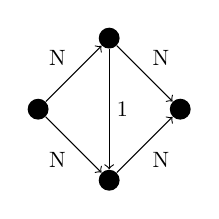
\begin{tikzpicture}
		\node[circle, fill, black, scale = .8] (A) {};
		\node[circle, fill, black, scale = .8, above right = 1cm of A] (B) {};
		\node[circle, fill, black, scale = .8, below right = 1cm of A] (C) {};
		\node[circle, fill, black, scale = .8, below right = 1cm of B] (D) {};
		
		\path (A) edge[->] node[above left, scale = .8]{N} (B);
		\path (A) edge[->] node[below left, scale = .8]{N} (C);
		\path (B) edge[->] node[right, scale = .8]{1} (C);
		\path (B) edge[->] node[above right, scale = .8]{N} (D);
		\path (C) edge[->] node[below right, scale = .8]{N} (D);
	\end{tikzpicture}
	\end{center}
\end{beispiel}
\begin{satz}[MaxFlow-MinCut]
	In einem Netzwerk $(G, u, s, t)$ ist der maximale Wert eines $s$-$t$-Flusses gleich der minimalen Kapazität eines $s$-$t$-Schnittes.
\end{satz}
\begin{proof}
	Satz 4.7 $\Rightarrow$ für jeden maximalen $s$-$t$-Fluss $f$ gibt es einen $s$-$t$-Schnitt dessen Kapazität gleich dem Flusswert ist $\Rightarrow~max~Wert(f) \ge~min~\text{Wert eines Schnittes} \overset{4.5~b)}{\Rightarrow}$ MaxFlow = MinCut. $Wert(f) \le \sum_{e\in \delta^+(A)}u(e)$
\end{proof}
\begin{beobachtung}
	Wollen wir den Wert eines maximalen Flusses erhöhen, müssen wir am minimalen Cut die Kapazitäten verändern.
\end{beobachtung}
\begin{korollar}
	Wenn die Kapazitäten in einem Netzwerk ganzzahlig sind, dann existiert ein optimaler ganzzahliger Fluss.
\end{korollar}
\begin{satz}
	Sei $(G, u, s, t)$ ein Netzwerk und $f$ ein $s$-$t$-Fluss in $G$. Dann gibt es
	\begin{itemize}
		\item eine Familie $P$ von $s$-$t$-Pfaden
		\item eine Familie $C$ von Kreisen
	\end{itemize}
	so dass \[f(e) = \sum_{p\in P \cup C: e \in E(p)}w(p), ~\forall~e\in E(G)\] und $\card{P} + \card{C}\le \card{E(G)}$. $\sum_{p\in P} w(p) = Wert(f)$. \\[5pt]
	Außerdem: Wenn $f$ ganzzahlig ist kann $w$ ganzzahlig gewählt werden.
\end{satz}
\begin{proof}
	Wir konstruieren $P, C$ und $w$ durch Induktion über die Anzahl der Kanten mit positivem Fluss. Sei $e=(v_0, w_0)$ eine Kante mit $f(e)>0$. Falls $w_0\neq t$ gibt es eine Kante $(v_0, w_1)$ mit positivem Fluss (Flusserhaltung). Wir machen immer weiter (mit $i=1$ startend) und finden ein $w_{i+1}$:\\
	Wenn $w_i\in \set{t, v_0, w_0, ..., w_{i-1}}$ stoppen wir (Muss passieren, da endliche Knotenzahl). Sonst finden wir Kante $(w_i, w_{i+1})$ mit positivem Fluss und setzen $i = i+1$.\\
	Das Gleiche machen wir in der anderen Richtung. Wir suchen sukzessive Vorgängerkanten: Falls $v_0 \neq s$, gibt es eine Kante $(v_1, v_0)$ mit positivem Fluss ... . Ende:
	\begin{enumerate}[label=\arabic*)]
		\item $w_i\in \set{v_0, w_0, ..., w_{i-1}}$ oder $v_j \in \set{w_0, v_0, ..., v_{j-1}}$ dann haben wir einen Kreis.
		\item $w_i=t$ und $v_j=s$, dann haben wir einen $s$-$t$-Pfad.
	\end{enumerate}
	Wir haben eine Kreis oder einen $s$-$t$-Pfad in $G$ gefunden. UND: wir haben nur Kanten mit positivem Fluss verwendet. Sei $p$ dieser Kreis oder Pfad. Sei $w(p) = \underset{e\in E(p)}{min}f(e)$.\\
	Setze \[f'(e):=\begin{cases}
		f(e) - w(p) &\text{für } e\in E(p),\\
		f(e) &\text{für } e\notin E(p).
	\end{cases}\]
	Das heißt wir entfernen einen Fluss in Höhe von $w(p)$ auf $p$. Dann können wir für $f'$ die Induktionsannahme verwenden (weniger Kanten mit positivem Fluss).
\end{proof}
\newpage
\begin{algorithm}
	\Input{Netzwerk $(G, u, s, t)$}
	\Output{Ein $s$-$t$-Fluss $f$ mit maximalem Wert}\vspace*{5pt}
	Setze $f(e)=0~\forall e\in A(G)$\\
	Finde einen kürzesten $f$-augmentierenden Pfad $P$\\
	\hspace*{15pt}Falls keiner existiert: \textbf{stop} \\
	Berechne $\gamma := \underset{e\in P}{min}~ u_f(e)$\\
	\hspace*{15pt}Augmentiere $f$ entlang $P$ um $\gamma$ und \textbf{goto} 2
	\caption{Edmonds-Karp Algorithmus (1972)}
	\label{fig:Algorithmus}
\end{algorithm}
\textit{Also: Implementiere 2. von Ford-Fulkerson als BFS in $G_f$}
\begin{lemma}
	Sei $f_1, f_2, ...$ eine Folge von Flüssen, wobei $f_{i+1}$ aus $f_i$ durch Augmentierung entlang eines kürzesten f-augmentierenden Pfades $P_i$ entsteht. Dann gilt:
	\begin{enumerate}[label=\alph*)]
		\item $\card{E(P_k)} \le \card{E(P_{k+1})} ~\forall~k$
		\item $\card{E(P_k)} + 2 \le \card{E(P_l)} ~\forall~k<l$, so dass $P_k \cup P_l$ ein Paar entgegengesetzer Kanten enthält.
	\end{enumerate}
\end{lemma}
\begin{proof}~\\
	zu a): Betrachte den Graphen $G_1$, den man aus $P_k \cup P_{k+1}$ durch entfernen von entgegengesetzen Kanten erhält (Kanten, die in $P_k$ und $P_{k+1}$ auftreten, werden zweifach aufgenommen). Jede Kante aus $E(G_{f_{k+1}})\setminus E(G_{f_k})$ muss eine Umkehrkante einer Kante in $P_k$ sein. $\Rightarrow E(G_1) \subseteq E(G_{f_k})$. Sei $H_1$ der Graph bestehend aus zwei Kopien von $(t,s) \Rightarrow G_1 + H_1$ ist eulersch $\Rightarrow$ Jeder Knoten wird genauso oft betreten wie verlassen $\Rightarrow G_1 + H_1$ lässt sich in Menge von Kantendisjunkte Kreise zerlegen. $\Rightarrow$ für jede Kante in $H_1$ gibt es einen Kantendisjunkten $s$-$t$-Pfad  $Q_1, Q_2$. $E(G_1) \subseteq E(G_{f_k}) \Rightarrow Q_1, Q_2$ sind $f_k$-augmentierende Pfade. $P_k$ kürzester $f_k$-augmentierender Pfad.\\
	$\Rightarrow \card{E(P_k)} \le \card{E(Q_1)}, \card{E(P_k)} \le \card{E(Q_2)}$.\\
	$\Rightarrow 2\card{E(P_k)} \le \card{E(Q_1)} + \card{E(Q_2)} \le \card{E(G_1)} \le \card{E(P_k)} + \card{E(P_{k+1})}$.\\
	$\Rightarrow \card{E(P_k)} \le \card{E(P_{k+1})}$.\\
	zu b): Wegen a) gilt auch $k < i \le l: \card{E(P_k)} \le \card{E(P_i)} \le \card{E(P_l)}$.\\
	Spezieller: Wir betrachten ein Paar $k,l$ mit $k < i \le l$ mit $P_i \cup P_l$ hat kein Paar entgegengesetzter Kanten. Wie oben: Sei $G_1$ der Graph, der aus $P_k \cup P_l$ durch Entfernen entgegengesetzter Kantenpaare entsteht. Wieder $E(G_1) \subseteq E(G_{f_k})$, $E(P_k) \subseteq E(G_{f_k})$, $E(P_l) \subseteq E(G_{f_k})$. Jede Kante in $E(G_{f_l}), E(G_{f_k})$ muss eine Umkehrung einer Kante in $P_k, ..., P_{l-1}$ sein. Aber (Wahl von $k$ und $l$) nur $P_k$ enthält Umkehrung von Kanten in $P_l$. Wieder:
	\begin{itemize}
		\item $H_1$ zwei Kopien von $(t,s)$\\
		$\hookrightarrow$ 2 kantendisjunkte $s$-$t$-Pfade $Q_1$ und $Q_2$
		\item $Q_1, Q_2$ beide $f_k$-augmentierende Pfade
	\end{itemize}
	$P_k$ war kürzester $f_k$-augmentierender Pfad.\\
	$\Rightarrow \card{E(P_k)} \le \card{E(Q_1)}, \card{E(P_k)} \le \card{E(Q_2)}$.\\
	$\Rightarrow 2\card{E(P_k)} \le \card{E(Q_1)} + \card{E(Q_2)} \le \card{G_1} -2 \le \card{E(P_k)} + \card{E(P_l)} - 2$ da wir mindestens 2 Kanten entfernt haben.
\end{proof}
\begin{satz}
	Unabhängig von den Kantenkapazitäten stoppt Algorithmus 10 (Edmonds-Karp) nach höchstens $\frac{m\cdot n}{2}$ Augmentierungen.
\end{satz}
\begin{proof}~
	\begin{itemize}
		\item[i)] Jede Augmentierung hat eine \dq Engstelle\dq, eine \dq Flaschenhalskante\dq, die den Wert $\gamma$, und damit den Wert um den der Fluss erhöht wird, begrenzt.
		\item[ii)] Eine Kante in $\overset{\leftrightarrow}{G}$ kann nur dann zweimal als Flaschenhalskante auftauchen, wenn zwischendurch die Gegenkante in einem augmentierenden Pfad vorgekommen ist (dann wird die Kante wieder in den Residualgraphen aufgenommen). Für eine Kante $e$ sei $P_{i_1}, P_{i_2}, ...$ die Folge von augmentierenden Pfaden, die $e$ als Flaschenhalskante enthalten $\to$ zwischen $P_{ij}$ und $P_{ij+1}$ gibt es einen augmentierenden Pfad $P_k ~(ij < k \le ij+1)$ der $\overset{\leftarrow}{e}$ enthält. $\overset{4.11~b)}{\Rightarrow} \card{E(P_{ij})} + 4 \le \card{E(P_k)} + 2 \le \card{E(P_{ij+1})} ~\forall j$. Wegen $1 \le \card{E(P_{ij})} \le n-1$ gilt $j < \frac{n}{4}$ also höchstens $\frac{n}{4}$ augmentierende Pfade enthalten $e$ als Flaschenhalskante. Jeder augmentierende Pfad, muss mindestens eine Kante aus $\overset{\leftrightarrow}{G}$ als Flaschenhalskante haben. $\Rightarrow$ Höchstens $\card{\underbrace{E(\overset{\leftrightarrow}{G})}_{2m}}\cdot \frac{n}{4} = \frac{n \cdot m}{2}$ augmentierende Pfade.
	\end{itemize}
\end{proof}
\begin{korollar}
	Der Edmonds-Karp Algorithmus löst MaxFlow in $O(m^2\cdot n)$.
\end{korollar}
\begin{proof}
	Satz 4.12 $\to ~\le\frac{m\cdot n}{2}$ Augmentierungen, je Augmentierung BFS $\to$ $O(m)$.
\end{proof}
	\section{Matching}
\begin{definition}[Matching]~
	\begin{itemize}
		\item[i)] Ein \textbf{Matching} in einem Grap $G=(V,E)$ ist eine Menge paarweise disjunkter Kanten.
		\item[ii)] Ein Matching heißt \textbf{perfekt}, wenn jeder Knoten in $V(G)$ zu einer Matchingkante gehört.
		\item[iii)] Ein \textbf{Vertex Cover} ist eine Kantenüberdeckende Knotenmenge.
		\item[iv)] \textbf{Maximales Matching} in $G:$ $\mathcal{V}(G)$.
		\item[v)] \textbf{Minimales Vertex Cover} in $G:$ $\mathcal{T}(G)$.
	\end{itemize}
\end{definition}
\begin{figure}[ht]
	\begin{subfigure}[c]{0.5\textwidth}
		\begin{center}
			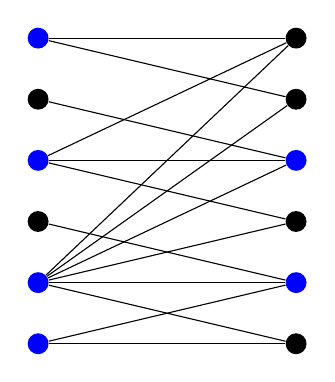
\begin{tikzpicture}
			\node[circle, fill, blue, scale = .8] (A) {};
			\node[circle, fill, black, scale = .8, below = 0.5cm of A] (B) {};
			\node[circle, fill, blue, scale = .8, below = 0.5cm of B] (C) {};
			\node[circle, fill, black, scale = .8, below = 0.5cm of C] (D) {};
			\node[circle, fill, blue, scale = .8, below = 0.5cm of D] (E) {};
			\node[circle, fill, blue, scale = .8, below = 0.5cm of E] (F) {};
			
			\node[circle, fill, black, scale = .8, right = 3cm of A] (H) {};
			\node[circle, fill, black, scale = .8, below = 0.5cm of H] (I) {};
			\node[circle, fill, blue, scale = .8, below = 0.5cm of I] (J) {};
			\node[circle, fill, black, scale = .8, below = 0.5cm of J] (K) {};
			\node[circle, fill, blue, scale = .8, below = 0.5cm of K] (L) {};
			\node[circle, fill, black, scale = .8, below = 0.5cm of L] (M) {};
			
			\path (A) edge (H);
			\path (A) edge (I);
			\path (B) edge (J);
			\path (C) edge (H);
			\path (C) edge (J);
			\path (C) edge (K);
			\path (D) edge (L);
			\path (E) edge (H);
			\path (E) edge (I);
			\path (E) edge (J);
			\path (E) edge (K);
			\path (E) edge (L);
			\path (E) edge (M);
			\path (F) edge (L);
			\path (F) edge (M);
			\end{tikzpicture}
		\end{center}
		\subcaption{Vertex Cover}
	\end{subfigure}
	\begin{subfigure}[c]{0.5\textwidth}
		\begin{center}
			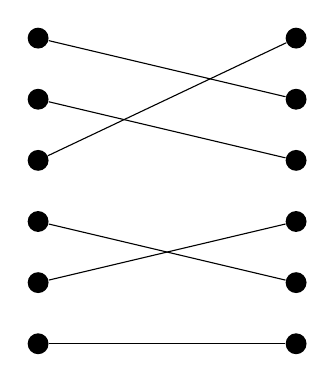
\begin{tikzpicture}[every loop/.style={}]
			\node[circle, fill, black, scale = .8] (A) {};
			\node[circle, fill, black, scale = .8, below = 0.5cm of A] (B) {};
			\node[circle, fill, black, scale = .8, below = 0.5cm of B] (C) {};
			\node[circle, fill, black, scale = .8, below = 0.5cm of C] (D) {};
			\node[circle, fill, black, scale = .8, below = 0.5cm of D] (E) {};
			\node[circle, fill, black, scale = .8, below = 0.5cm of E] (F) {};
			
			\node[circle, fill, black, scale = .8, right = 3cm of A] (H) {};
			\node[circle, fill, black, scale = .8, below = 0.5cm of H] (I) {};
			\node[circle, fill, black, scale = .8, below = 0.5cm of I] (J) {};
			\node[circle, fill, black, scale = .8, below = 0.5cm of J] (K) {};
			\node[circle, fill, black, scale = .8, below = 0.5cm of K] (L) {};
			\node[circle, fill, black, scale = .8, below = 0.5cm of L] (M) {};
			
			\path (A) edge (I);
			\path (B) edge (J);
			\path (C) edge (H);
			\path (D) edge (L);
			\path (E) edge (K);
			\path (F) edge (M);
			\end{tikzpicture}
		\end{center}
		\subcaption{Matching}
	\end{subfigure}
	\caption{Vertex Cover und Matching im bipartiten Graph}
\end{figure}
\begin{problem}[Kardinalitätsmatching/Max Matching]~\\[5pt]
	\hspace*{10pt}\textbf{Gegeben: }Ungerichteter Graph $G = (V,E)$.\\[5pt]
	\hspace*{10pt}\textbf{Gesucht: }Ein Matching $M$ größtmöglicher Kardinalität.
\end{problem}
\begin{problem}[Minimales Vertex Cover]~\\[5pt]
	\hspace*{10pt}\textbf{Gegeben: }Ungerichteter Graph $G = (V,E)$.\\[5pt]
	\hspace*{10pt}\textbf{Gesucht: }Ein Vertex Cover $C$ kleinstmöglicher Kardinalität.
\end{problem}
\begin{satz}
	Sei $G$ ein ungerichteter Graph. Es gilt max Matching $\le$ min Vertex Cover.
\end{satz}
\begin{figure}[ht]
	\begin{center}
		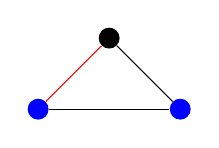
\begin{tikzpicture}
			\node[circle, fill, black, scale = .8] (A) {};
			\node[circle, fill, blue, scale = .8, below left = 1cm of A] (B) {};
			\node[circle, fill, blue, scale = .8, below right = 1cm of A] (C) {};
			
			\path (A) edge[red] (B);
			\path (A) edge (C);
			\path (B) edge (C);
		\end{tikzpicture}
		\end{center}
	\caption{max Matching $\le$ min Vertex Cover}
\end{figure}
\newpage
\subsection{Bipartites Matching}
\begin{definition}[Bipartite Graphen]
	Ein Graph heißt \textbf{bipartit}, wenn sich die Knotenmenge so in zwei Mengen $A,B$ mit $V(G) = A \dot\cup B$ zerlegen lässt, dass jede Kante genau einen Knoten in $A$ und einen Knoten in $B$ enthält.
\end{definition}
\textit{Damit: Bipartite Graphen enthalten keine Kreise ungerader Länge. Für bipartite Graphen gibt es eine Beziehung zu Flussproblemen:}
\begin{center}
	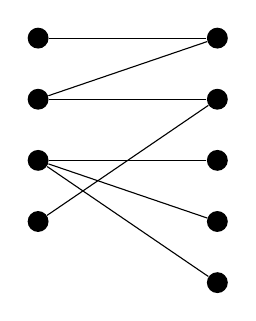
\begin{tikzpicture}
		\node[circle, fill, black, scale = .8] (A) {};
		\node[circle, fill, black, scale = .8, below = .5cm of A] (B) {};
		\node[circle, fill, black, scale = .8, below = .5cm of B] (C) {};
		\node[circle, fill, black, scale = .8, below = .5cm of C] (D) {};
		
		\node[circle, fill, black, scale = .8, right = 2cm of A] (E) {};
		\node[circle, fill, black, scale = .8, below = .5cm of E] (F) {};
		\node[circle, fill, black, scale = .8, below = .5cm of F] (G) {};
		\node[circle, fill, black, scale = .8, below = .5cm of G] (H) {};
		\node[circle, fill, black, scale = .8, below = .5cm of H] (I) {};
		
		\path (A) edge (E);
		\path (B) edge (E);
		\path (B) edge (F);
		\path (C) edge (G);
		\path (C) edge (H);
		\path (C) edge (I);
		\path (D) edge (F);
	\end{tikzpicture}
\end{center}
\textit{
\begin{itemize}
	\item füge 2 neue Knoten $s,t$ ein: Kanten von $s$ nach $v\in A$ und von $v\in B$ zu $t$.
	\item Kanten von $A$ nach $B$ richten.
	\item $u(e) = 1$ falls $s\in e$ oder $t\in e$, $u(e) = \infty$ sonst.
\end{itemize}
}
\begin{center}
	\begin{tikzpicture}
	\node[circle, fill, black, scale = .8, below left = 1.5cm of A, label = s] (S) {};
	\node[circle, fill, black, scale = .8] (A) {};
	\node[circle, fill, black, scale = .8, below = .5cm of A] (B) {};
	\node[circle, fill, black, scale = .8, below = .5cm of B] (C) {};
	\node[circle, fill, black, scale = .8, below = .5cm of C] (D) {};
	
	\node[circle, fill, black, scale = .8, below right = 1.5cm of E, label = t] (T) {};
	\node[circle, fill, black, scale = .8, right = 2cm of A] (E) {};
	\node[circle, fill, black, scale = .8, below = .5cm of E] (F) {};
	\node[circle, fill, black, scale = .8, below = .5cm of F] (G) {};
	\node[circle, fill, black, scale = .8, below = .5cm of G] (H) {};
	\node[circle, fill, black, scale = .8, below = .5cm of H] (I) {};
	
	\path (A) edge[->] node[above, scale = .8]{$\infty$} (E);
	\path (B) edge[->] node[above, scale = .8]{$\infty$} (E);
	\path (B) edge[->] node[above, scale = .8]{$\infty$} (F);
	\path (C) edge[->] node[above, scale = .8]{$\infty$} (G);
	\path (C) edge[->] node[above, scale = .8]{$\infty$} (H);
	\path (C) edge[->] node[above, scale = .8]{$\infty$} (I);
	\path (D) edge[->] node[above, scale = .8]{$\infty$} (F);
	\path (S) edge[->] node[above, scale = .8]{1} (A);
	\path (S) edge[->] node[above, scale = .8]{1} (B);
	\path (S) edge[->] node[above, scale = .8]{1} (C);
	\path (S) edge[->] node[above, scale = .8]{1} (D);
	\path (E) edge[->] node[above, scale = .8]{1} (T);
	\path (F) edge[->] node[above, scale = .8]{1} (T);
	\path (G) edge[->] node[above, scale = .8]{1} (T);
	\path (H) edge[->] node[above, scale = .8]{1} (T);
	\path (I) edge[->] node[above, scale = .8]{1} (T);
	\end{tikzpicture}
\end{center}
\textit{Aus gegebenen bipartiten Graph $G$ wird $(G',u,s,t)$.}
\begin{satz}
	Ein bipartites Matching maximaler Kardinalität in $G$ entspricht einem maximalen Fluss in $(G',u,s,t)$ und umgekehrt.
\end{satz}
\begin{proof}~
	\begin{itemize}
		\item Jedes Matching in $G$ lässt sich direkt auf einen Fluss in $G'$ abbilden, indem die Matchingkanten einen Fluss von jeweisl 1 erhalten und entsprechende Flüsse von $s$ und $t$ gewählt werden.
		\item Umgekehrt lässt sich jeder ganzzahliger Fluss (der auf jeder Kante den Wert 0 oder 1 hat) auf ein Matching in $G$ abbilden.
	\end{itemize}
	Da es immer ein ganzzahliges Optimum für das Flussproblem gibt, sind also insbesondere die Optimalwerte gleich.
\end{proof}
\begin{satz}
	In bipartiten Graphen gilt $\mathcal{V}(G) = \mathcal{T}(G)$.
\end{satz}
\begin{proof}
	$\mathcal{V}(G) = Max~Flow(G) = Min~Cut(G) \overset{!}{=} \mathcal{T}(G)$. 
		\begin{figure}[ht]
			\begin{center}
				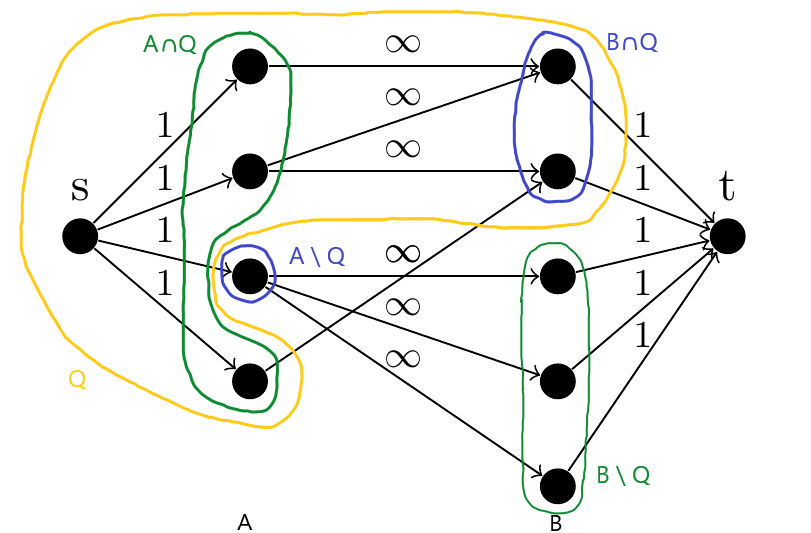
\includegraphics[scale=.3]{images/satz_5_8.png}
			\end{center}
		\end{figure}\\
	Betrachte Min Cut $\delta^+(\set{s}\cup Q), Q \subseteq V$. Dieser Cut hat endliche Kapazität, d.h. es gibt keine Kante von $A \cap Q$ zu $B\setminus Q$.
	\begin{eqnarray*}
		A \cap Q & \text{ zu } & B \cap Q\\
		A \cap Q & \text{ zu } & B \setminus Q ~\lightning\\
		A \setminus Q & \text{ zu } & B \cap Q\\
		A \setminus Q & \text{ zu } & B \setminus Q
	\end{eqnarray*}
	Also ist jede Kante in $G$ inzident zu einem Knoten aus $C = (A\setminus Q)\cup (B \cap Q)$. D.h. $C$ ist ein Cover der Größe $\card{C} = \card{A\setminus Q} + \card{B\cap Q}$. Die Kapazität des Cuts ist ebenfalls $\card{C} = \card{A\setminus Q} + \card{B\cap Q}$ (nach Konstruktion) d.h. Min Cut = min Vertex Cover.
\end{proof}
\begin{satz}[Satz von Hall]
	Sei $G$ ein bipartiter Graph mit $V(G)=A\dot\cup B$. Dann hat $G$ ein $A$ überdeckendes Matching $\Leftrightarrow$ $\card{\underbrace{T(X)}_{\mathclap{\text{Menge der Nachbarn von } X}}} \ge \card{X}~\forall X\subseteq A$.
\end{satz}
\begin{proof}~
	\begin{itemize}
		\item Notwendigkeit ist klar.
		\item Um zu zeigen, dass auch hinreichend nehmen wir an $G$ hat kein $A$ überdeckendes Matching. $\mathcal{V}(G) \le \card{A} \overset{5.7}{\Rightarrow} \mathcal{T}(G) < \card{A}$. Sei $A' \subseteq A, B' \subseteq B$, so dass $A' \cup B'$ alle Kanten überdeckt und $\card{A' \cup B'} < \card{A} \Leftrightarrow \card{A'} + \card{B'} < \card{A}$ (da $A'$ und $B'$ disjunkt) $\Leftrightarrow \card{B'} < \card{A} - \card{A'}$. Es gilt $T(A\setminus A') \subseteq B'$ ( da $B'$ alle Kanten überdeckt, die nicht von $A'$ überdeckt werden) $\Rightarrow \card{T(A\setminus A')} \le \card{B'} < \card{A} - \card{A'} = \card{A\setminus A'}~\lightning$ Kontraposition der Hinrichtung gezeigt.
	\end{itemize}
\end{proof}
\begin{korollar}[Heiratssatz von Frobenius]
	Sei $G$ ein bipartiter Graph mit $V(G) = A\dot\cup B$. Dann hat $G$ ein perfektes Matching $\Leftrightarrow \card{A}=\card{B}$ und $\card{T(X)} \ge \card{X}~\forall X \subseteq A$.
\end{korollar}
\textit{Aus dem Beweis von Satz 5.7 folgt}
\begin{korollar}
	Das Kardinalitätsmatching-Problem kann in bipartiten Graphen in $O(n\cdot m)$ gelöst werden.
\end{korollar}
\begin{proof}
	Konstruktion von oben. Betrachte Ford-Fulkerson für das äquivalente Flussproblem
	\begin{itemize}
		\item Eine Augmentierung benötigt $O(m)$.
		\item Um einen maximalen $s$-$t$-Fluss (und damit ein maximales Matching) zu finden brauchen wir höchstens $n$ Augmentierungen $\Rightarrow$ $(O(m\cdot n))$.
	\end{itemize}
\end{proof}
\textit{Wie sehen Augmentierungen aus?\\
\hspace*{10pt}$\hookrightarrow$ Verbesserung von Matchings}
\begin{figure}[ht]
	\begin{center}
	\begin{tikzpicture}
	\node[circle, fill, black, scale = .8, below left = 1.5cm of A, label = s] (S) {};
	\node[circle, fill, black, scale = .8] (A) {};
	\node[circle, fill, black, scale = .8, below = .5cm of A] (B) {};
	\node[circle, fill, black, scale = .8, below = .5cm of B] (C) {};
	\node[circle, fill, black, scale = .8, below = .5cm of C] (D) {};
	
	\node[circle, fill, black, scale = .8, below right = 1.5cm of E, label = t] (T) {};
	\node[circle, fill, black, scale = .8, right = 2cm of A] (E) {};
	\node[circle, fill, black, scale = .8, below = .5cm of E] (F) {};
	\node[circle, fill, black, scale = .8, below = .5cm of F] (G) {};
	\node[circle, fill, black, scale = .8, below = .5cm of G] (H) {};
	
	\path (A) edge[->] (E);
	\path (B) edge[->, red] (E);
	\path (B) edge[->] (F);
	\path (C) edge[->] (G);
	\path (C) edge[->, red] (F);
	\path (D) edge[->, red] (G);
	\path (D) edge[->] (H);
	\path (S) edge[->] (A);
	\path (S) edge[->] (B);
	\path (S) edge[->] (C);
	\path (S) edge[->] (D);
	\path (E) edge[->] (T);
	\path (F) edge[->] (T);
	\path (G) edge[->] (T);
	\path (H) edge[->] (T);
	
	\path (S) edge[->, green, bend left] (A);
	\path (A) edge[->, green, bend left] (E);
	\path (E) edge[->, green, bend right] (B);
	\path (B) edge[->, green, bend left] (F);
	\path (F) edge[->, green, bend right] (C);
	\path (C) edge[->, green, bend left] (G);
	\path (G) edge[->, green, bend right] (D);
	\path (D) edge[->, green, bend right] (H);
	\path (H) edge[->, green, bend right] (T);
	\end{tikzpicture}
	\caption{augmentierender Pfad in $G'$}
	\end{center}
\vspace*{-10pt}
\end{figure}\\
\textit{Augmentierende Pfade in $(G',u,s,t)$ entsprechen alternierenden Pfaden in $G$.}
\begin{definition}
	Sei $G$ ein Graph (bipartit oder nicht), und sei $M$ ein beliebiges Matching in $G$. Ein Pfad $P$ ist ein \textbf{$M$-alternierender Pfad}, wenn $E(P)\setminus M$ ein Matching ist. Ein $M$-alternierender Pfad ist \textbf{$M$-augmentierend}, wenn seine Endpunkte nicht von $M$ überdeckt werden (er zwei nicht gematchte Knoten verbindet).
\end{definition}
\textit{Augmentierende Pfade müssen ungerade Länge haben.}
\begin{figure}[ht]
	\begin{center}
	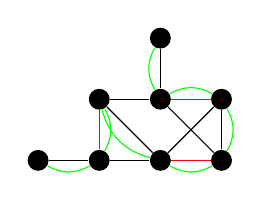
\begin{tikzpicture}
	\node[circle, fill, black, scale = .8] (A) {};
	\node[circle, fill, black, scale = .8, right = .5cm of A] (B) {};
	\node[circle, fill, black, scale = .8, right = .5cm of B] (C) {};
	\node[circle, fill, black, scale = .8, right = .5cm of C] (D) {};
	\node[circle, fill, black, scale = .8, above = .5cm of B] (E) {};
	\node[circle, fill, black, scale = .8, above = .5cm of C] (F) {};
	\node[circle, fill, black, scale = .8, above = .5cm of D] (G) {};
	\node[circle, fill, black, scale = .8, above = .5cm of F] (H) {};
	
	\path (A) edge[-] (B);
	\path (B) edge[-] (C);
	\path (C) edge[-, red] (D);
	\path (B) edge[-, red] (E);
	\path (E) edge[-] (F);
	\path (E) edge[-] (C);
	\path (F) edge[-, red] (G);
	\path (F) edge[-] (H);
	\path (G) edge[-] (D);
	\path (G) edge[-] (C);
	\path (F) edge[-] (D);
	
	\path (A) edge[-, bend right, green] (B);
	\path (C) edge[-, bend right, green] (D);
	\path (B) edge[-, bend right, green] (E);
	\path (E) edge[-, bend right, green] (C);
	\path (F) edge[-, bend left, green] (G);
	\path (F) edge[-, bend left, green] (H);
	\path (G) edge[-, bend left, green] (D);
	\end{tikzpicture}
	\caption{$M$-augmentierender Pfad}
	\end{center}
\end{figure}
\newpage
\begin{satz}[Berg, 1957]
	Sei $G$ ein Graph mit einem beliebigen Matching $M$. $M$ hat max Kardinalität $\Leftrightarrow$ es gibt keinen $M$-augmentierenden Pfad.
\end{satz}
\begin{proof}~\\
	\glqq$\Rightarrow$\grqq: Sei $P$ ein $M$-augmentierender Pfad $\Rightarrow M \Delta E(P)~ (=(M\setminus E(P)) \cup (E(P)\setminus M))$ ist Matching größterer Kardinalität la $M$. $\Rightarrow M$ ist nicht maximal.\\
	\glqq$\Leftarrow$\grqq: Sei $M'$ ein Matching mit $\card{M'} > \card{M} \Rightarrow M \Delta M'$ ist kantendisjunkte Vereinigung alternierender Kreise und Pfade. Wegen $\card{M'} > \card{M}$ muss mindestens einer dieser Pfade $M$-augmentierend sein.
\end{proof}
\textit{Wie findet man einen $M$-augmentierende Pfad?
\begin{itemize}
	\item Matchingkanten (schwarz)
	\item Nicht-Matchingkanten (weiß)
	\item \glqq suchende\grqq~ Knoten (weiß)
	\item \glqq gleichgültige\grqq~ Knoten (schwarz)
\end{itemize}
Starte bei einem ungematchten Knoten $v \to$ \glqq weiß\grqq.\\
Falls einer der Nachbarknoten ungematcht\\
\hspace*{10pt}$\hookrightarrow$ Füge Kante hinzu, liefert besseres Matching\\
Falls alle gematcht $\to$ alle \glqq schwarz \grqq; daran: \glqq schwarze\grqq~ Kanten\\
\hspace*{10pt}$\hookrightarrow$ andere Endknoten}
\begin{center}
	\begin{tikzpicture}
	\node[circle, fill, black, scale = .8, label = v] (A) {};
	\node[circle, fill, black, scale = .8, right = 1cm of A] (B) {};
	\node[circle, fill, black, scale = .8, above = .5cm of B] (C) {};
	\node[circle, fill, black, scale = .8, below = .5cm of B] (D) {};
	
	\node[state, scale = .35, right = 1cm of B] (E) {};
	\node[state, scale = .35,, above = .5cm of E] (F) {};
	\node[state, scale = .35,, below = .5cm of E] (G) {};
	
	\node[state, scale = .35,, right = 1cm of G] (H) {};
	
	\path (A) edge[-] (B);
	\path (A) edge[-] (C);
	\path (A) edge[-] (D);
	\path (B) edge[-, red] (E);
	\path (C) edge[-, red] (F);
	\path (D) edge[-, red] (G);
	\path (G) edge[-, dotted] (H);
	\end{tikzpicture}
\end{center}
\textit{Falls einer der weißen Knoten anderweitig \glqq versorgbar\grqq~ ist entsteht ein ungerader alternierender Pfad, also eine Verbesserung des Matchings.\\
Falls nicht: Färbe Endknoten wieder weiß und fahre fort.\\
$\Rightarrow$ Baumstruktur\\
\hspace*{10pt}$\hookrightarrow$ weiße\textbackslash schwarze Knoten abwechselnd\\
\hspace*{10pt}$\hookrightarrow$ weiße\textbackslash schwarze Kanten abwechselnd\\
$\Rightarrow$ Breitensuche von $v$ aus\\
\hspace*{10pt}$\hookrightarrow$ Für jede ZhK von $G$ wähle einen ungematchten Knoten $r$ als Wurzel\\
\hspace*{10pt}$\hookrightarrow$ Wir nennen einen Knoten \glqq schwarz\grqq, wenn er ungeraden Abstand von $r$ hat; \hspace*{23pt}\glqq weiß\grqq, wenn er geraden Abstand von $r$ hat\\
Mit BFS bauen wir einen alternierenden Wald.}
\begin{algorithm}
	\Input{$G=(V,E)$ mit $V=V_1 \dot\cup V_2$}
	\Output{Maximales Matching $M$}\vspace*{5pt}
	Setze $M=\emptyset, R=\emptyset$\\
	\While{$\exists r\in V_1\setminus R$ ungematcht}{
		Wähle $r\in V_1\setminus R$ ungematcht\\
		Setze $T:=(\set{r}, \emptyset)$\\
		$R:= R \cup \set{r}$\\
		$W(T) = \set{r}$\\
		\While{$\exists \set{v,w} \in E$ mit $v \in W(T) \wedge w\notin V(T)$}{
			\eIf{$w$ ist ungematcht}{
				Benutze $\set{v,w}$ um augmentierenden Pfad zu komplettieren\\
				\hspace*{10pt}$\hookrightarrow$ augmentiere $M$\\
				\If{es gibt keinen ungematchten Knoten mehr}{
					\textbf{return} \glqq Perfektes Matching\grqq				
				}
				\textbf{goto} 2
			}{
				Benutze $\set{v,w}$ um $T$ zu erweitern
			}
		}
	}
	\textbf{return} Maximales Matching $M$
	\caption{Maximales Matching in bipartiten Graphen}
	\label{fig:Algorithmus}
\end{algorithm}
\begin{algorithm}
	\Input{Matching $M$ in Graph $G$,\\ $M$-alternierender Baum $T$,\\ Kante $\set{v,w}$ von $G$ mit $v\in W(T), w \notin V(T)$, $w$ ist gematcht}
	Sei $\set{w,z}$ die Matchingkante, die $w$ überdeckt\\
	Ersetze $T$ durch $E(T) = E(T)\cup \set{\set{v,w}, \set{w,z}}, W(T) = W(T) \cup \set{z}$
	\caption{Benutze $\set{v,w}$ um $T$ zu erweitern}
	\label{fig:Algorithmus}
\end{algorithm}
\begin{center}
	\begin{tikzpicture}
	\node[circle, fill, black, scale = .8, label = r] (A) {};
	\node[circle, fill, black, scale = .8, right = 1cm of A] (B) {};
	\node[circle, fill, black, scale = .8, above = .5cm of B] (C) {};
	\node[circle, fill, black, scale = .8, below = .5cm of B] (D) {};
	
	\node[state, scale = .35, right = 1cm of B] (E) {};
	\node[state, scale = .35, above = .5cm of E] (F) {};
	\node[state, scale = .35, below = .5cm of E, label = v] (G) {};
	
	\node[circle, fill, black, scale = .8, right = 1cm of G, label = w] (H) {};
	\node[state, scale = .35, right = 1cm of H, label = z] (I) {};
	
	\path (A) edge[-] (B);
	\path (A) edge[-] (C);
	\path (A) edge[-] (D);
	\path (B) edge[-, red] (E);
	\path (C) edge[-, red] (F);
	\path (D) edge[-, red] (G);
	\path (G) edge[-] (H);
	\path (H) edge[-, red] (I);
	\end{tikzpicture}
\end{center}
\begin{satz}
	Algorithmus 11 liefert ein korrektes Ergebnis.
\end{satz}
\begin{proof}
	Satz 5.12 in Verbindung mit Bipartitheit von $G$.
\end{proof}
\begin{beobachtung}
	Für perfekte Matchings brauchen wir eine gerade Anzahl an Knoten. Reicht aber nicht aus.
\end{beobachtung}
\begin{satz}[Satz von Tutte, 1947]
	Ein Graph $G=(V,E)$ hat ein perfektes Matching $\Leftrightarrow$ für jede Menge $A \subseteq V$ gilt $\underbrace{OC}_{\mathclap{\text{\# ungerader Komponenten}}}(G\setminus A) \le \card{A}$.
\end{satz}
\begin{satz}[Tutte-Berg-Formel, 1958]
	Für $G=(V,E)$ gilt:
	\begin{equation*}
		max\set{\card{M}~\vert~ M \text{ ist Matching}} = min\set{\frac{1}{2}(\card{V}-OC(G\setminus A) + \card{A})~\vert~ A \subseteq V}
	\end{equation*}
\end{satz}
\begin{satz}
	Sei $G$ bipartit, $M$ ein Matching, $T$ ein alternierender Baum für den keine Kante von $G$ einen Knoten in $W(T)$ mit einem Knoten nicht in $V(T)$ verbindet. Dann hat $G$ kein perfektes Matching.
\end{satz}
\begin{proof}
	Sei $S(T) = V(T)\setminus W(T)$, die Menge der schwarzen Kanten in $T$. Nach Konstruktion gilt $\card{S(T)} = \card{W(T)} - 1$. $G$ ist bipartit.\\
	$\Rightarrow$ keine 2 weißen Knoten können benachbart sein.\\
	$\Rightarrow$ jeder Knoten in $W(T)$ ungerade Komponente (Kardinalität 1) von $G\setminus S(T)$.\\
	$\underset{\card{S(T)} < \card{W(T)}}{\overset{5.15}{\Rightarrow}}$ Behauptung.
\end{proof}

\end{document}
